É bastante usual que as pessoas tenham contato com lógica em algum momento da
vida. Este contato é, em geral, com a Lógica Proposicional Básica.
Esta lógica estuda argumentos cuja validade depende das noções de ``se-então'',
``e'', ``ou'', ``não'', além de noções similares. Estas noções definem os
operadores mais usuais da lógica. 

A Linguagem Proposicional é, portanto, uma formalização que provê regras
específicas para construção de argumentos e testes de validade que utilizam
estas noções~\cite{gensler}. A especificação apresentada neste documento,
utiliza consoantes minúsculas para representar afirmações at\^omicas, ou seja,
uma proposição que pode ser verdadeira ou falsa. Os operadores utilizados estão
expressos na Tabela~\ref{tab:operadores_prop}.

\begin{table}[!tbh]
\label{tab:operadores_prop}
\caption{Operadores da Lógica Proposicional}
\begin{center}
\begin{tabular}{|rcl|}
   \hline  
   $\neg p$ & $:=$ & $\text{não}\ p$ \\
   $p \wedge q$ & $:=$ & $p\ \text{e}\ q$ \\
   $p \vee q$ & $:=$ & $p\ \text{ou}\ q$ \\
   $p \then q$ & $:=$ & se $p$ então $q$ \\
   $p \iff q$ & $:=$ & $p$ se, e somente se, $q$ \\
   \hline
\end{tabular}
\end{center}
\end{table}

Os operadores podem ser combinados entre si e com símbolos at\^omicos (ou
proposicionais) para formar fórmulas. As fórmulas que pertencem a Linguagem
Proposicional, são as bem formadas, ou seja, que expressam um significado, como
definido a seguir:

\begin{definition}
   As fórmulas bem formadas da Linguagem Proposicional são definidas
   recursivamente como segue:
   \begin{itemize}
       \item [(i)] Os símbolos proposicionais $(p,q,\ldots)$ são fórmulas bem formadas
   \end{itemize}
   Agora considere que $\varphi$ e $\psi$ são fórmulas bem formadas. Então:
   \begin{itemize}
       \item [(ii)] $\neg \varphi$
       \item [(iii)] $\varphi \wedge \psi$
       \item [(iv)] $\varphi \vee \psi$
       \item [(v)] $\varphi \then \psi$
       \item [(vi)] $\varphi \iff \psi$
   \end{itemize}
   também são fórmulas bem formadas.
\end{definition}

Observe que é possível representar equivalências entre os operadores, conforme
exemplos na Tabela~\ref{tab:equivalencia}.  Neste sentido, os operadores $\neg$
e $\vee$ são suficientes para expressar toda a Lógica Proposicional. Os demais
são utilizados para facilitar a leitura e diminuir o tamanho das fórmulas.

\begin{table}[!h]
\label{tab:equivalencia}
\caption{Equivalência entre operadores}
\begin{center}
\begin{tabular}{|rcl|}
   \hline  
   $\neg (p \vee q)$ & $=$ & $\neg p \wedge \neg q$ \\
   $p \then q$ & $=$ & $\neg p \vee q$ \\
   $p \iff q$ & $=$ & $(p \then q) \wedge (q \then p)$ \\
   \hline
\end{tabular}
\end{center}
\end{table}

Agora já podemos começar a raciocinar sobre algum mundo possível utilizando
Lógica Proposicional. 

Seja, então, $t$ o planeta em que vivemos. É possível escrever diversas
afirmações que podem ter valoração verdadeira ou falsa e é possível combiná-las
para escrever argumentos. Considere as afirmações contidas na
Figura~\ref{fig:prop}.

\begin{figure}[!tbh]
\label{fig:prop}
\begin{center}
\begin{tabular}{|l|}
   \hline  
   $p:$ O céu é azul.\\
   $r:$ O Brasil fica na América do Sul.\\
   $s:$ Machado de Assis nasceu no Brasil.\\
   $v:$ Machado de Assis nasceu na América do Sul.\\
   $z:$ A Argentina fica na Ásia.\\
   $q:$ Buenos Aires é a capital da Argentina.\\
   $l:$ Buenos Aires fica na Ásia.\\
   \hline
\end{tabular}
\end{center}
\caption{Exemplos de afirmações sobre o nosso planeta}
\end{figure}

Sabemos que $p,r,s,v$ e $q$ são verdadeiras e que $z$ e $l$ são falsas. Observe
os argumentos descritos na Figura~\ref{fig:argumentos_prop}. 

\begin{figure}[!tbh]
\label{fig:argumentos_prop}
\begin{center}
    \begin{tabular}{ccc}
        \begin{tabular}{|r|}
            \hline
            Premissas:\\
            $r$\\
            $s$\\
            \hline
            Conclusão:\\
            $v$\\
            \hline
        \end{tabular}
        &
        \begin{tabular}{|r|}
            \hline
            Premissas:\\
            $p$\\
            $q$\\
            \hline
            Conclusão:\\
            $z$\\
            \hline
        \end{tabular}
        &
        \begin{tabular}{|r|}
            \hline
            Premissas:\\
            $z$\\
            $q$\\
            \hline
            Conclusão:\\
            $l$\\
            \hline
        \end{tabular} \\
        (a) & (b) & (c)
    \end{tabular}
\end{center}
\caption{Exemplos de argumentos sobre as afirmações da Figura~\ref{fig:prop}}
\end{figure}

Conforme a definição de validade vista no começo desta seção, podemos concluir
que (a) e (c) são argumentos válidos, e (b) é um argumento inválido. Vale
lembrar que estes argumentos estão definidos no Planeta Terra ($t$), então
podemos esboçar um modelo que satisfaz os argumentos válidos, conforme
Figura~\ref{fig:modelos_prop}.

\begin{center}
\begin{figure}
\label{fig:modelos_prop}
\begin{center}
\begin{tabular}{cc}
\begin{tikzpicture}
\matrix[nodes={draw,thick, minimum size=1.5cm},
row sep=0.3cm,column sep=1.5cm,ampersand replacement=\&] {
    \node[circle,label=150:$t$](w0) {$
        \begin{array}{c}       
            r\quad s\\
            v
        \end{array}
    $}; \\
};

\end{tikzpicture}
&
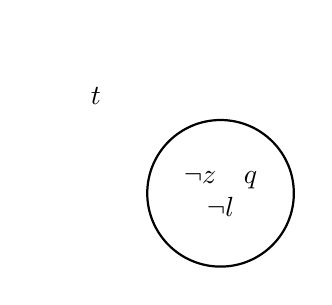
\begin{tikzpicture}
\matrix[nodes={draw,thick, minimum size=1.5cm},
row sep=0.3cm,column sep=1.5cm,ampersand replacement=\&] {
    \node[circle,label=150:$t$](w0) {$
        \begin{array}{c}       
            \neg z\quad q\\
            \neg l
        \end{array}
    $}; \\
};

\end{tikzpicture} \\
(a) & (c)
\end{tabular}
\end{center}
\caption{Modelos que satisfazem os argumentos (a) e (c) da
Figure~\ref{fig:argumentos_prop}}
\end{figure}
\end{center}

FAZER O LINK DE ARGUMENTOS PARA FÓRMULAS

